\chapter{Evaluation}
\label{chap:evaluation}

We now evaluate our model through a series of microbenchmarks, system benchmarks and case studies on
a both and ARM and x86 hardware.
First, we present the hardware platforms used in addition to the cost of timer operations on those
platforms. Then we demonstrate the minimal performance overhead of our mechanisms using a set of 
microbenchmarks which measure the overheads of the MCS kernel versus the existing \selfour kernel, 
which is referred to as \emph{baseline}.  

We then run a several system benchmarks, first comparing a Redis~\citep{redis:url} 
implementation to baseline \selfour, Linux and NetBSD to show that our kernel is competitive.
We then demonstrate temporal
isolation between threads sharing the same CPU in two scenarios,
using Redis again, followed by ipbench~\citep{Wienand_Macpherson_04}. Finally, we show isolation in a
shared encryption server, and measure the cost of various timeout fault handling policies. 

In addition, we evaluate two user-level scheduler implementations: one which implements a static
criticality switch, and a user-level \gls{EDF} implementation which we show is
competitive with an in-kernel \gls{EDF} scheduling from \litmus. Lastly, we use an \gls{IPC}
throughput benchmark to demonstrate minimal, multicore scalability overhead, and we show 
how resource server threads can migrate between processing cores.

\section{Hardware}

% describe benchmark setup, details of each hardware platform
We ran microbenchmarks on a variety of hardware to show the overheads of the model compared to
baseline \selfour. \Cref{t:evaluation-hardware} summarises the hardware platforms. \textsc{Sabre} is
the verified platform for \selfour, although at the time of writing verification for \textsc{x64} is
ongoing. Currently, the only platforms that support more than one core are \textsc{Sabre},
and \textsc{x64}.

Two of our platforms, \textsc{x64} and \textsc{Hikey} support both 32- and 64-bit execution modes.
We use both, referring to them as \textsc{ia32} and \textsc{Hikey32} when in 32-bit mode and
\textsc{x64} and \textsc{Hikey64} otherwise. All platforms have out of order execution, except
\textsc{Hikey}, which is in-order.

Additionally, we use several load generators running Linux on an isolated network for 
benchmarks that require a network.

\begin{table}[ht]
\begin{tabularx}{\textwidth}{Xlrrrrr}\toprule
    \emph{Platform}       & \emph{Microarch.} & \emph{Clock } & L1 & L2 & L3  & TLB  \\
    \emph{Arch}           & \emph{CPU}        & GHz           & (KiB) & (KiB) & (MiB) & (entries) \\\midrule
    \textsc{KZM} (32-bit) & ARM1136JF-S       & 1.0           & 16       & 128      & \no      & 32\\
    \small{ARMv6}                 & i.MX31            &               & 4$\times$        & 8$\times$         & \no      & 2$\times$  \\
    \rowcolor{gray!25}
    \textsc{Sabre} (32-bit) & Cortex-A9       & 1.0           & 32+32    & 1024     & \no      & 64\\
    \rowcolor{gray!25}
    \small{ARMv7}                    & i.MX6             &               & 4$\times$  & 16 $\times$  & \no & 2$\times$  \\
    \textsc{Hikey} (64-bit)  & Cortex-A53        & 1.2           & 32+32     & 512 & \no & 128         \\
    \small{ARMv8}                    & Kirin 620         &               & 4+2$\times$       & 16$\times$    & \no   & 4$\times$  \\
    \rowcolor{gray!25}
    \textsc{TX1}   (64-bit)  & Cortex-A57        & 1.9           &  32+48 & 2,048 & \no & 256          \\
    \rowcolor{gray!25}
    \small{ARMv8}                   & Jetson TX1  &                   & 2+3$\times$       & 16$\times$ & \no & 4$\times$ \\
    \textsc{x64}    (64-bit) & i7-4770           & 3.1           & 32+32 & 256 & 8 & 128,8 \\          
    \small{x86}                     & Haswell            &                 & 8$\times$ & 8$\times$ & 16$\times$ & 8$\times$ \\
    \bottomrule
\end{tabularx}
    \caption{Hardware platform details, ``$\times$`` is associativity, and + indicates i-cache+d-cache.}
\label{t:evaluation-hardware}
\end{table}

\section{Overheads}

We first present a suite of microbenchmarks to evaluate any performance overheads against baseline
\selfour.
For each benchmark we ensure \gls{FPU} context switching is off by performing the required number of 
system calls 
without activating it such that the kernel will cease switching the FPU context. We present
overheads on IPC operations, signalling and interrupts, and finally scheduling. 

For each of the benchmarks in this section, we measure the cost of measurement, which is reading the
cycle counter on ARM platforms, and the \gls{TSC} on x86, and subtract the value obtained
from the final result.

\subsection{Timer}
\label{s:eval-timer}

Two of the main sources of overhead introduced by our model are related to the need to read and
reprogram the timer on non-fastpath kernel entries, and when performing a scheduling context switch.
We show the results of microbenchmarks of both of these operations in \Cref{t:evaluation-timer}, and
note the timer hardware used on the specific platform. 

\begin{table}[ht]\centering
\rowcolors{2}{gray!25}{white}
\begin{tabularx}{\textwidth}{lXccc}\toprule
    \emph{Platform} & \emph{Timer} & \emph{Read time} & \emph{Set timeout} & \emph{Sum}
    \\\midrule
    \textsc{KZM}               & General purpose timer    & 83 (0)   & 203(0)  & 286   \\
    \textsc{Sabre}             & ARM MPCore global timer  & 23 (0)   & 36 (0)  & 59    \\
    \textsc{Hikey32/64}        & ARM generic timers       &  6 (0)   &  6 (0)  & 12    \\
    \textsc{TX1}               & ARM generic timers       &  8 (0)   &  1 (0)  & 9     \\
    \textsc{ia32}              & TSC deadline mode        & 12 (2.2) & 220 (1.0) & 232 \\
    \textsc{x64}               & TSC deadline mode        & 11 (2.3) & 217 (2.0) & 228 \\
    \bottomrule\hline
\end{tabularx}
\caption{Latency of timer operations per platform in cycles. Standard deviations shown
in parentheses.}
\label{t:evaluation-timer}
\end{table}

For both microbenchmarks, we read the timestamp before and after the operation, and do this 102
times, discarding the first two results to prime the cache.  We take the difference of the cycle
counts, and subtract the cost of measuring the cycle counter itself. The results show the cost of
both operations separately, and then their sum, which is the total measured overhead introduced by timers on
scheduling context switch.

All platforms excluding \textsc{KZM} have a 64-bit timer available, making \textsc{KZM} the only
platform requiring timer overflow interrupts, which are not measured as \textsc{KZM} is a deprecated
platform provided for comparison with modern ARM versions.

\textsc{Sabre} and \textsc{KZM} both use memory mapped timers, the 32-bit general purpose timer for
the former and 64-bit ARM global timer for the latter. \textsc{Sabre} has four cores and the timer
registers are banked, making access fast for each core. Timer access on \textsc{Sabre} is
significantly faster than the \textsc{KZM}. 

For all other ARM platforms, the ARM generic timers are available, which are accessed via the
coprocessor. The majority of new ARM platforms support the generic timers. 

On \textsc{x64} we use the \gls{TSC} with \gls{TSC}-deadline
mode~\citep{Intel_64_IA-32:asdmspg_325384}, an architectural \gls{MSR} available since
Intel SandyBridge by which a local-APIC timer interrupt is triggered when the \gls{TSC} matches the
programmed value. 

\Cref{t:evaluation-timer} shows the instruction latency of each timer operation. In practice, especially
for \textsc{x64}, these operations are subject to pipeline parallelism and out-of-order execution, which
reduces the overhead.

Results on both architectures show that the overhead of a tickless kernel, which requires the timers
to be frequently read and reprogrammed, is practical on modern hardware. On ARM, timer costs have
reduced by an order of magnitude from ARMv6 through to ARMv8. 

\subsection{IPC performance}

\Gls{IPC} performance is a critical measure of the practicality and efficiency of a
microkernel~\citep{Liedtke_95}. We benchmark our \gls{IPC} operations against base system, \selfour,
which has an established efficient \gls{IPC} fastpath~\citep{Elphinstone_Heiser_13}. 

To evaluate IPC performance we set up a client (the caller) and server (the callee) in different
address spaces. We take timestamps on either side of the IPC operation being benchmarked and record
the difference. This is done 16 times for each result value to prime the cache, then record the next
value. Results presented are for performing this a total of 16 times. Additionally, we measure the
overhead of system calls stubs in the same way and subtract this from the measurement, to obtain
only the kernel cost of the operation\footnote{The \gls{IPC} benchmarks already existed for
 \selfour, but we modified them to support the \gls{MCS} kernel as part of this thesis}.
    The message sent is zero length, so neither the caller or callee's \gls{IPC} buffer accessed.
    This is done for both directions of IPC, as described in \Cref{sec:seL4-api}. 

We evaluate the \gls{IPC} fastpath and two slowpath variants: slowpath between passive threads and
active threads.

\subsubsection{Fastpath}

\begin{table}[ht]\centering
\begin{tabular}{ll r@{~}l r@{~}l r@{~}r}\toprule
\emph{Platform}           & \multicolumn{1}{c}{\emph{Operation}}
                                & \multicolumn{2}{c}{\emph{Baseline}}
                                & \multicolumn{2}{c}{\emph{MCS     }}
                                & \multicolumn{2}{c}{\emph{Overhead}} \\
    \ipcmicro{KZM}{kzm}{fastpath}
    \ipcmicro{Sabre}{sabre}{fastpath}
    \ipcmicro{Hikey32}{hikey32}{fastpath}
    \ipcmicro{Hikey64}{hikey64}{fastpath}
    \ipcmicro{TX1}{tx1}{fastpath}
    \ipcmicro{x64}{haswell}{fastpath}
    \ipcmicro{ia32}{ia32}{fastpath}
    \bottomrule
\end{tabular}
\caption{Time in cycles for \selfour fastpath \gls{IPC}.}
\label{t:fastpath-ipc-micro}
\end{table}

% TODO update below paragraph
Fastpath results for \call and \replyrecv increase by a few percent on each platform,
resulting from extra checks on the fastpath to
accommodate scheduling contexts, an extra capability lookup for the Resume object, touching two
separate new objects (\gls{SCO} and Resume object) and enforcing priorities
on IPC delivery (baseline does \gls{FIFO}).


We look at each platform in detail to determine the source of the overhead by using the performance
monitor unit. 

\subsubsection{Slowpath}
\label{eval:slowpath}

% TODO rewrite with all platforms
Slowpath results show the greater cost of the model, as shown in \cref{t:slowpath-ipc-micro}, 
which shows the cost of a slowpath \gls{IPC} between two passive threads. 

The benchmark hits the slowpath as the priorities are arranged such that the task starting the
operation is a lower priority, which means not only do we invoke the slowpath but also the
scheduler. However, since the server is passive, we do not change scheduling context, meaning the
only overhead on \call is unnecessarily reading the time on kernel entry, as well as the mechanisms
for scheduling context donation. This is quite small, very small on \textsc{x64} (1\%) as the kernel simply
does a non-serialised read of the \gls{TSC}. On ARM the overhead is greater (8\%), as we use the
ARM Cortex-A9 MPCore global timer (the only 64-bit timer available on the platform), which is memory
mapped and shared between all of the cores. We evaluate the cost of reading the timer with a hot cache 
for ARM as 23 cycles. 

\replyrecv shows a higher overhead on both platforms, due to the extra slowpath capability lookup of
the resume capability, the ordered IPC checks, and accessing the \gls{SCO} and resume object.

\begin{table}[ht]\centering
\begin{tabular}{ll r@{~}l r@{~}l r@{~}r}\toprule
\emph{Platform}           & \multicolumn{1}{c}{\emph{Operation}}
                                & \multicolumn{2}{c}{\emph{Base}}
                                & \multicolumn{2}{c}{\emph{MCS}}
                                & \multicolumn{2}{c}{\emph{Overhead}}\\
    \ipcmicro{KZM}{kzm}{slowpath}
    \ipcmicro{Sabre}{sabre}{slowpath}
    \ipcmicro{Hikey32}{hikey32}{slowpath}
    \ipcmicro{Hikey64}{hikey64}{slowpath}
    \ipcmicro{TX1}{tx1}{slowpath}
    \ipcmicro{x64}{haswell}{slowpath}
    \ipcmicro{ia32}{ia32}{slowpath}
    \bottomrule
\end{tabular}
\caption{Time in cycles \selfour slowpath \gls{IPC} between passive threads.}
\label{t:slowpath-ipc-micro}
\end{table}

\subsubsection{Active slowpath}

Finally, we show the cost of slowpath IPC between two active threads, where both caller and
callee have a scheduling context. In addition to the
overheads of \cref{eval:slowpath}, we must bill and change the scheduling context and reprogram the
timer. On \textsc{x64}, reprogramming the timer uses \gls{TSC}-deadline mode, which is programmed via the
model specific registers and is also very fast. On ARM, we evaluate the cost of reprogramming the timer
with a hot cache as 36 cycles. 
%TODO what the hell is the rest of the overhead
% get instruction counts
% get branch mispredict etc

\begin{table}[hb]\centering
\begin{tabular}{cl r@{~}l r@{~}l r@{~}r}\toprule
\emph{Platform}           & \multicolumn{1}{c}{\emph{Operation}}
                                & \multicolumn{2}{c}{\emph{Base}}
                                & \multicolumn{2}{c}{\emph{MCS}}
                                & \multicolumn{2}{c}{\emph{Overhead}} \\
    \ipcmicro{KZM}{kzm}{slowpath-active}
    \ipcmicro{Sabre}{sabre}{slowpath-active}
    \ipcmicro{Hikey32}{hikey32}{slowpath-active}
    \ipcmicro{Hikey64}{hikey64}{slowpath-active}
    \ipcmicro{TX1}{tx1}{slowpath-active}
    \ipcmicro{x64}{haswell}{slowpath-active}
    \ipcmicro{ia32}{ia32}{slowpath-active}
    \bottomrule
\end{tabular}
\caption{Time in cycles for \selfour slowpath \gls{IPC} between active threads.}
\label{t:slowpath-ipc-active-micro}
\end{table}

\subsection{Faults}

Recall that fault handling in \selfour occurs via an \gls{IPC} simulated by the kernel to a fault
endpoint, which a fault handling thread blocks on, waiting for any fault messages
(\cref{api:faults}). 

To measure the fault handling cost, we run two threads in the same address space: a fault handler
and a faulting thread, with the same priority.
We trigger a fault by executing an undefined instruction in a loop on the faulting thread's
side. The fault handler then increments the instruction pointer past the undefined
instruction, and the benchmark continues. The fault handler is passive, so no scheduling context
switch occurs. 

We measure both directions of the fault, both the round trip cost of from the fault  handlers
side. Similar to standard slowpath-IPC, the largest impact is on the reply path, where ordered IPC
and the extra lookup of the resume object add overhead.

\begin{table}[ht]\centering
\begin{tabular}{cl r@{~}l  r@{~}l r@{~}r}\toprule
\emph{Platform}           & \multicolumn{1}{c}{\emph{Operation}}
                                & \multicolumn{2}{c}{\emph{Baseline}}
                                & \multicolumn{2}{c}{\emph{MCS}}
                                & \multicolumn{2}{c}{\emph{Overhead}} \\ 
    % no kzm, fault benchmark doesn't work
    \faultmicro{Sabre}{sabre}
    \faultmicro{Hikey32}{hikey32}
    \faultmicro{Hikey64}{hikey64}
    \faultmicro{TX1}{tx1}
    \faultmicro{x64}{haswell}
    \faultmicro{ia32}{ia32}
    \bottomrule
\end{tabular}
\caption{Time in cycles of \selfour fault \gls{IPC} between passive threads.}
\label{t:slowpath-fault-micro}
\end{table}

\subsection{Signalling and interrupts}

We measure interrupt latency using two threads, one spinning in a loop
updating a volatile cycle counter, the other, higher priority thread
waiting for an interrupt. On delivery, the handler thread determines the
interrupt latency by subtracting the
looped timestamp from the current time. The overhead is higher here as we must switch scheduling
contexts, which requires reprogramming the timer, however the scheduler is by-passed as the switch
is to a higher priority thread.


\begin{table}[h]\centering
\begin{tabular}{cl r@{~}l r@{~}l r@{~}r}\toprule
\emph{Platform}           & \multicolumn{1}{c}{\emph{Operation}}
                                & \multicolumn{2}{c}{\emph{Base}}
                                & \multicolumn{2}{c}{\emph{MCS}}
                                & \multicolumn{2}{c}{\emph{Overhead}} \\
    \irqmicro{KZM}{kzm}
    \irqmicro{Sabre}{sabre}
    \irqmicro{Hikey32}{hikey32}
    \irqmicro{Hikey64}{hikey64}
    \irqmicro{TX1}{tx1}
    \irqmicro{x64}{haswell}
    \irqmicro{ia32}{ia32}
    \bottomrule
\end{tabular}
\caption{Time in cycles of \selfour signal and IRQ latency on \selfour baseline vs. MCS kernels. Standard deviations
shown in brackets.}
\label{t:micro-irq}
\end{table}

The \code{signal()} operation signals a Notification object (semaphore). This microbenchmark
evaluates the cost of signalling a lower priority thread, a common operation for interrupt service
routines. We have added an experimental fastpath to both the base and \gls{MCS} kernels, which shows
that when the scheduler is not used and a thread switch does not occur, there is no overhead at all.

\subsection{Scheduling}

\begin{table}[ht]\centering
\begin{tabular}{cl r@{~}l  r@{~}l r@{~}r}\toprule
\emph{Platform}           & \multicolumn{1}{c}{\emph{Operation}}
                                & \multicolumn{2}{c}{\emph{Base}}
                                & \multicolumn{2}{c}{\emph{MCS}}
                                & \multicolumn{2}{c}{\emph{Overhead}} \\

    
    \schedulemicro{KZM}{kzm}
    \schedulemicro{Sabre}{sabre}
    \schedulemicro{Hikey32}{hikey32}
    \schedulemicro{Hikey64}{hikey64}
    \schedulemicro{TX1}{tx1}
    \schedulemicro{x64}{haswell}
    \schedulemicro{ia32}{ia32}
    \bottomrule
\end{tabular}
\caption{Time in cycles of \selfour IPC scheduling costs.}
\label{t:micro-schedule}
\end{table}

The \code{schedule} benchmark measures the cost of a signal to a higher priority thread, which forces 
a reschedule operation.
Scheduling cost increases noticeably due to the need for first reading
and then reprogramming the timer for budget enforcement. Furthermore,
the sporadic replenishment logic is far more complicated than the
previous tick-based logic, and there is some extra code for
dealing with scheduling contexts. Note that \selfour IPC,
particularly scheduler-context donation (and its predecessor, the
undisciplined timeslice donation), is designed to minimise the need for
invoking the scheduler, therefore this increase is unlikely to have
a noticeable effect in practice. 

\subsection{Full system benchmark}
\label{s:evaluation-redis-overhead}

To demonstrate the impact of the overheads in a real system scenario, 
we measure the performance of the Redis key value store~\citep{redis:url} using 
\gls{YCSB}~\citep{Cooper_STRS_10} on baseline and MCS \selfour, and compare this
against Linux, the Rump unikernel~\citep{Kantee_Cormack_14} and 
NetBSD~\citep{NetBSD:url} all on the \textsc{x64} machine.

For \selfour, we use a single-core Rump library OS~\citep{Kantee_Cormack_14} to provide 
NetBSD~\citep{NetBSD:url} network drivers at user level, by leveraging an existing port of this infrastructure
to \selfour~\citep{McCleod:be}.
The system consists of Redis/Rump running on three active \selfour threads: 
two for servicing interrupts (network, timer) and one for Rump, as shown in
\cref{f:redis-arch}. Interrupt threads run at the highest priority,
followed by Redis and a low-priority idle thread (not shown) for measuring CPU utilisation;
this setup forces frequent invocations of the scheduler and interrupt path.

 \begin{figure}[ht]
    \centering
    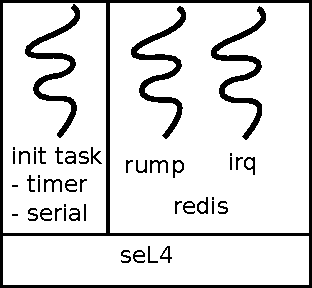
\includegraphics{redis-arch}
    \caption{System architecture of the Redis / \gls{YCSB} benchmark on \selfour, 
        Linux, NetBSD and Rump unikernel.}
    \label{f:redis-arch}
\end{figure}

\autoref{t:redis} shows the achieved throughput of Redis+Rump
running  bare-metal (BMK), and Redis on the seL4 baseline and as well as the MCS
branch, plus Linux and NetBSD (7.0.2) for comparison.

The table indicates the interrupt handling method used, as there is no single method supported
across all four scenarios. BMK only supports the legacy
programmable interrupt controller (PIC),
while NetBSD only supports message-signalled interrupts (MSI). Linux and seL4 both support the
advanced PIC (APIC).


The utilisation figures show that the system is fully loaded, except
in the Linux case, where there is a small amount of idle time. The
cost per operation (utilisation over throughput) is best on Linux, a
result of its highly optimised drivers and network stack. Our
bare-metal and \selfour-based setups use Rump's NetBSD drivers, and
actually performance within a few percent of native NetBSD. This
indicates that the MCS model comes with low overhead.

\begin{table}[t]\centering
      \rowcolors{3}{}{gray!25}
      \begin{tabularx}{\textwidth}{Xrrrrr}\toprule
          \emph{System}   & \emph{IRQ} & \emph{Throughput} & \emph{Utilisation} & \emph{Cost} & \emph{Latency} \\
                          &            & (k ops/s)         & (\%)               & per op.     & (ms)            \\
        \midrule

      \input{data/ycsb-redis.inc}
      \bottomrule
    \end{tabularx}
    \caption{Throughput (k\,ops/s) achieved by Redis using the YCSB
      workload A with 2 clients.  Latency is the average Read and Update,
      standard deviations in parentheses and omitted where less than the least
      significant digit shown.}
    \label{t:redis}
\end{table}

\section{Temporal Isolation}

We have demonstrated our model has little overhead and is competitive with existing monolithic
kernels. Now we evaluate temporal isolation properties, between processes and in a shared-server
scenario. 
In addition, we evaluate and demonstrate different
techniques to restore server state after a timeout exception.

% Show isolation between processes using different scheduling contexts
\subsection{Process isolation} 

We evaluate process isolation, where processes do not share resources, indirectly via network
throughput and network latency in two separate benchmarks. Note that the Rump unikernel only
currently supports x86 platforms, consequently these experiments are only carried out on
the \textsc{x64} platform. 

\subsubsection{Network throughput}

First, we demonstrate our isolation properties with the Redis architecture described in
\Cref{s:evaluation-redis-overhead} with an additional, high-priority active CPU-hog thread
competing for \gls{CPU} time.  All scheduling contexts in the system are configured with a
5\,ms period. We use the budget of the hog to control the amount of time left over
for the server configuration. \autoref{f:redis} shows the throughput
achieved by the YCSB-A workload as a function of the available CPU
bandwidth (i.e \ the complement of the bandwidth granted to the hog
thread). All data points are the average of three benchmark runs.

\begin{figure}[h]
  \centering
  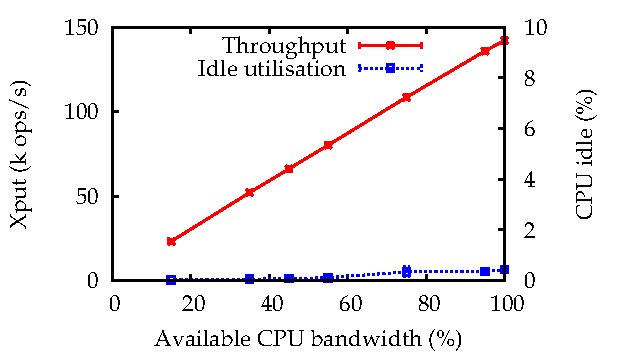
\includegraphics{redis}
  \caption{Throughput of Redis YCSB workload A and idle time versus available bandwidth.}
  \label{f:redis}
\end{figure}

The graph shows that the server is CPU limited (as indicated by very low idle time)
and consequently throughput scales linearly with available CPU
bandwidth.

\subsubsection{Network latency}

Second, we evaluate process isolation via network latency in a system shown in \cref{f:ipbench-arch}. 
The system consists of a single-core of a Linux \gls{VM} which runs at a high priority with a
constrained budget and a \gls{UDP} echo server running at a lower priority,
representing a lower-rate \textsc{high} thread. We
measure the average  and maximum UDP latency reported by the
ipbench~\citep{Wienand_Macpherson_04} latency test.

\begin{figure}[h]
    \centering
    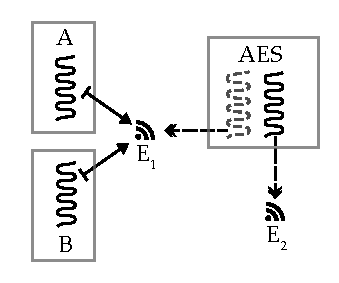
\includegraphics{ipbench-arch}
    \caption{System architecture of ipbench benchmark.}
    \label{f:ipbench-arch}
\end{figure}


Specifically, the Linux VM interacts with timer (PIT) and serial device drivers implemented as
passive servers outside the \gls{VM}; all three components are at a high priority. In the Linux server we
run a program (\code{yes > /dev/null}) which consumes all available
CPU bandwidth.  The UDP echo server, completely isolated from the Linux instance during the
benchmark, but sharing the
serial driver, runs at a low priority with its own HPET timer
driver.

Two client machines run ipbench daemons to send packets to the UDP-echo server on the target machine
(\textsc{x64}). The control machine, one of the load generators, runs ipbench with a \gls{UDP} socket at 10\,Mbps over a 1\,Gb/s Ethernet connection with 100-byte packets. The Linux VM has a 10\,ms period and we vary the
budget between 1\,ms and 9\,ms.
We represent the zero-budget case by an unconstrained Linux that is not running any user code.
Any time not consumed by Linux is available to UDP echo for processing
10,000 packets per second, or 100 packets in the time left over from
each of Linux's 10\,ms period.

\autoref{f:ipbench} shows the average and maximum \gls{UDP} latencies for
ten runs at each budget setting. We can see that the maximum latencies
follow exactly the budget of the Linux server (black line) up to 9\,ms. Only
when Linux has a full budget (10\,ms), and thus able to monopolise the
processor, does the UDP server miss its deadlines, resulting in a
latency spike.  This result shows that our sporadic server implementation is effective in bounding
interference of a high-priority process.

\begin{figure}[h]
  \centering
  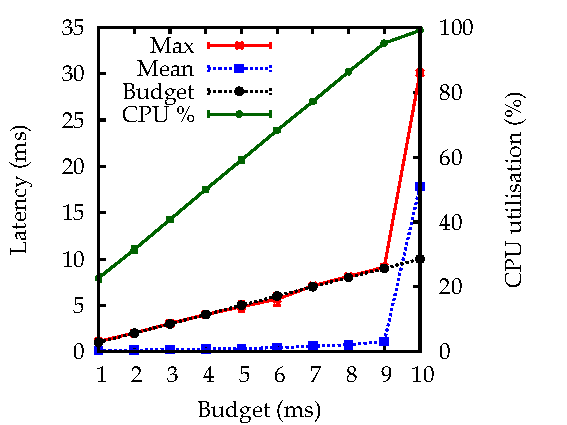
\includegraphics{ipbench}
  \caption{Average and maximum latency of UDP packets with a CPU hog running a high priority with a 10\,ms budget.}
  \label{f:ipbench}
\end{figure}

% Show isolation in a shared server
\subsection{Server isolation} 
\label{s:server-isolation}

To demonstrate temporal isolation in a shared server, we use a case study of an encryption service
using \gls{AES} to encrypt client data. We measure both the overhead of different
recovery techniques, and the throughput achieved when two clients constantly run out of budget in the server. 
We port an existing, open-source \gls{AES} implementation to a shared server running on \selfour, and run
benchmarks on both \textsc{x86} and \textsc{Sabre}.

\Cref{f:aes-arch} shows the architecture of the case study. Both clients $A$ and $B$ are single
 threaded and exist in separate address spaces to the server. The server has two threads, a passive
 thread for serving request on the clients scheduling context and an active thread which handles
 timeout exceptions for the server. The server and timeout exception handler share the same virtual
 memory and capability spaces.

\begin{figure}
\centering
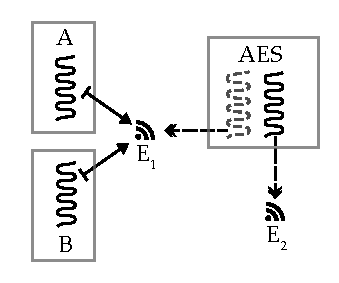
\includegraphics{aes-arch}
\caption{Architecture of the \gls{AES} case study. Client $A$ and $B$ make \gls{IPC} requests over
endpoint $E_{1}$ of passive $AES$ which has an active timeout fault handling thread waiting for
fault \gls{IPC} messages on endpoint $E_{2}$.}
\label{f:aes-arch}
\end{figure}

The server itself runs the AES-256 algorithm with a block size of 16~bytes. The server alternates between two
buffers, using an atomic swap, of which one always contains consistent state, the other is
dirty during processing. When a timeout fault occurs, only the dirty buffer is lost due to
inconsistency. Both clients request 4\,MiB of data to be encrypted, and have a budget insufficient to
complete the request. When the server is running on the clients scheduling context and the budget
expires, a timeout exception, which is a fault IPC message from the kernel, is delivered to the timeout
handler. 

\subsection{Timeout handling techniques}

If client scheduling context is depleted while the server is servicing the request, a timeout fault
is raised and sent to the timeout handler.  The appropriate protocol for handling such faults
depends ultimately on the requirements of the system.  Consequently, we implement and evaluate four
different timeout fault handling techniques: rollback, error, emergency and extend. 

While each technique is evaluated separately, combinations of such techniques could be used for
different clients depending on their requirements. For example, trusted clients may get special
treatment. Note that in all cases of blocking IPC, clients must trust the server as discussed in
\cref{s:locking}. Additionally, although out experiment places 
the timeout fault handler in the server's address
space, this is not necessary: for approaches that require access to scheduling contexts and
scheduling control capabilities, the timeout handler may be placed in a scheduling servers address
space, separate from the server itself.

\subsubsection{Rollback}

Rollback restores the server to the last known consistent state recorded. In the case of non-thread
safe servers, this may require rolling back an entire request. However, algorithms like \gls{AES}
which can easily be batched can make progress. The process for rollback involves is as follows:

\begin{enumerate}\label{e:rollback}
    \item A timeout fault is received by timeout handler, $T$ over $E_{2}$.
    \item $T$ constructs a reply message to the client from the last clean state, and sends this 
        message to the client by invoking the resume capability that the server has used for that client. 
        Because the resume object tracks the donation, the client's scheduling context is returned.
    \item $T$ then restores the server, $S$ to a known state by the timeout handler (restoring registers,
        stack frames and any global state). $S$ is restored to the point before it made its
        last system call, usually an \nbsendrecv, which it used to indicate to the initialiser that
        $S$ should be made passive, as part of the passive server initialisation protocol presented
        in \cref{sec:impl-passive-servers}.
    \item Now the server must return to blocking on the IPC endpoint, $E_{1}$. $T$ binds a
        scheduling context to $S$ and waits for a message. 
    \item Now the $S$ runs from its checkpoint, repeating the \nbsendrecv, signalling to $T$ that it
        can now be converted to passive once more and blocking on $E_{1}$. 
    \item $T$ wakes and converts the server back to passive.
    \item Finally, $T$ blocks on $E_{2}$, ready for further timeout faults.
\end{enumerate}

The rollback technique requires the server and timeout handler to both have access to the reply
object that the server is using, and the servers \gls{TCB}, meaning the timeout handler must be
trusted by the server. In our example the server and timeout handler run at the same priority, in
all cases both must run at higher priorities than the clients. 

Once the budget of the faulting client is replenished, it can then continue the request based on the
content of the reply message sent by the timeout handler. Clients are guaranteed progress as long as
their budget is sufficient to complete a single batch of progress.

If rollback is not suitable, the server can be similarly reset to the initial state and an error
returned to the client. However, this does not guarantee progress for clients with insufficient
budgets.

\subsubsection{Kill}

In cases of non-preemptible servers, potentially due to a lack of thread safety, one option is to
kill client threads. Such a scenario would stop untrusted misbehaving clients from constantly
monopolising server time.  We implement an example were the timeout handler has access to client \gls{TCB}
capabilities and simply calls suspend, however the server could also switch to a new reply object
and leave the client blocked forever, without access to any of the clients capabilities. 

The process for suspending the client is the same as that for \Cref{e:rollback} but for two aspects;
the server state does not need to be altered by the timeout handler as the server always 
restores to the same place, instead of replying to the client it is suspended.

\subsubsection{Emergency}

Another technique gives the server a one-off emergency budget to finish the client request, after
which the exception handler resets the server to being passive. This could be used in low
criticality \gls{SRT}
scenarios where isolation is desired but transient overruns are expected.
An example emergency protocol follows:

\begin{enumerate}\label{e:emergency}
    \item A timeout fault is received by timeout handler, $T$ over $E_{2}$.
    \item $T$ unbinds the client scheduling context from $S$.
    \item $T$ binds a new scheduling context to the $S$, which acts as an emergency budget.
    \item $T$ then replies to the timeout fault, resuming $S$.
    \item Now $T$ enqueues itself on $E_{1}$, such that when the server finishes the blocked request,
        $T$, being a higher priority, is served next.
    \item $S$ completes the request and replies to the client.
    \item $S$ receives the request from $T$, and replies immediate as it is an empty request.
    \item $T$ wakes, and converts the server back to passive.
    \item Finally $T$ blocks on $E_{2}$, ready for further timeout faults.
\end{enumerate}

This case requires the timeout handler to have access to client scheduling contexts in order to
unbind them from the server. 

\subsubsection{Extend}

The final technique is to simply increase the clients budget on each timeout, which requires the
timeout fault handler to have access to the clients scheduling contexts.
This could be deployed in \gls{SRT} systems or for specific threads with unknown budgets up to a limit. 

\begin{enumerate}\label{e:extend}
    \item A timeout fault is received by timeout handler, $T$ over $E_{2}$.
    \item $T$ extends the client's budget by configuring scheduling context.
    \item $T$ replies to the fault message, which resumes $S$.
\end{enumerate}

\subsection{Results}

We measure the pure handling overhead in each case, from when the timeout handler wakes up to when
it blocks again.  Given the small amount of rollback state, this measures the baseline overhead. For
schedulability analysis, the actual cost of the rollback would have to be added, in addition to the
duration of the timeout fault IPC. 
 
We run each benchmark with hot caches (primed by some warm-up
iterations)  as well as cold (flushed) caches and measure the 
latency of timeout handling, from the time the handler wakes up
until it replies to the server.

\autoref{t:rollback} shows the results. The maximum
cold-cache cost, which is relevant for schedulability analysis, differs by a factor of 3--4 between
the different recovery scenarios, indicating that all are about equally feasible.  Approaches that
restart the server and send \glspl{IPC} messages on its behalf (rollback, reply) are the most
expensive as they must restore the server state from a checkpoint and follow the passive server
initialisation protocol (recall \autoref{s:passive}). 

\begin{table}[t]\centering
\begin{tabular}{cllrrrr}\toprule
\emph{Platform} & \emph{Operation} & \emph{Cache} & \emph{Min} &
                          \emph{Max} & \emph{Mean} &
                          \multicolumn{1}{c}{\boldmath \(\sigma\)} \\\midrule
                          \multirow{8}{*}{\textsc{Sabre}} 
                          \input{data/generated/sabre-aes.inc} 
                          \midrule
                          \multirow{8}{*}{\textsc{x64}}
                          \input{data/generated/haswell-aes.inc}
                          \bottomrule
\end{tabular}
\caption{Cost of timeout handler operations in \(\mu\)s, as measured
  by timeout exception handler. \(\sigma\) is the standard deviation.}
\label{t:rollback}
\end{table}

\subsection{Rollback isolation}

We next demonstrate temporal isolation in the server by using the rollback
technique and measuring the time taken to encrypt 10 requests of 4\,MiB of
data. \autoref{f:aes} shows the result with both clients having the same
period, which we vary between 10\,ms and 1000\,ms.
In each graph we vary the clients' budgets between 0 and the
period. The extreme ends are special, as one of the clients has a full
budget and keeps invoking the server without ever getting rolled back,
thus monopolising the processor. In all other cases, each client
processes at most 4\,MiB of data per period, and either succeeds (if
the budget is sufficient) or is rolled back after processing less than 4\,MiB.

\begin{figure*}[t]
  \centering
  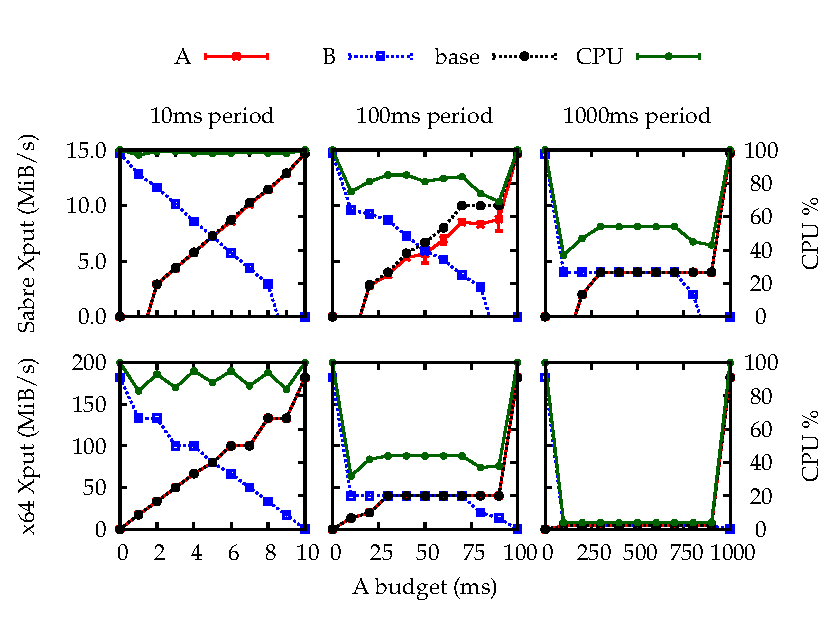
\includegraphics{aes-shared}
  \caption{Throughput for clients A and B of a passive AES server processing 10 requests of 4\,MiB of data with
      limited budgets on the \textsc{x64} (top row) and \textsc{Sabre} (bottom row) platforms. The two clients' budgets
      add up to the period, which is varied between graphs (10, 100, 1000\,ms). Clients sleep when
      they process each 4\,MiB, until the next period, except when their budgets are full. Each data point is the average of 10 runs, error bars show the standard deviation.}
  \label{f:aes}
\end{figure*}


The results show that in the CPU-limited cases (left graphs)
we have the expected near perfect proportionality between throughput and
budget (with slight wiggles due to the rollbacks), showing isolation between clients. In the cases where there is headspace (centre of the right
graphs), both clients achieve their desired throughput.

\section{Practicality}

Fundamental to the microkernel philosophy is keeping policy out of the
kernel as much as possible, and instead providing general mechanisms
that allow the implementation of arbitrary policies
\citep{Heiser_Elphinstone_16}.  As on the face of it, our
fixed-priority-based model seems to violate this principle,  we
demonstrate that the model is general enough to support the efficient
implementation of alternate policies at user level. Specifically, we
implement two user-level schedulers: first, a static mixed criticality
scheduler~\citep{Baruah_BD_11}, which we also compare to an in-kernel
implementation and secondly an \gls{EDF} scheduler, which we compare to \litmus.

\subsection{Criticality}

Static, mixed-criticality, fixed-priority schedulers are based on \emph{mode
switches}, which effectively mean altering the priority of threads in bulk:
critical threads that may be of low rate are bumped higher than their
low-criticality counter parts, to ensure deadlines are met in exceptional
circumstances. 

We implement a kernel mechanism for changing priorities in bulk of threads 
and compare with a user-level approach which simply changes the priority of threads
one at a time. In our prototype implementation, the kernel tracks all threads of specific criticalities and boosts their priority on a made switch. However, given threads are kept in per-priority queues, each thread must be removed and reinserted into a new queue, so either way the complexity of the mode-switch is $O(n)$. 

\begin{figure}
  \centering
  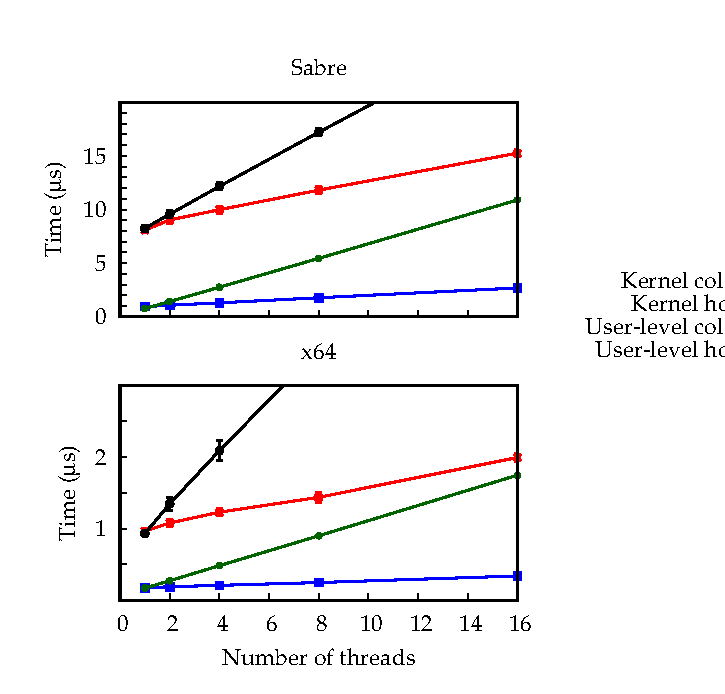
\includegraphics[width=\linewidth]{mode-switch-all}
  \caption{Cost of switching the priority of $n$ threads in kernel and user level, with hot
            and cold caches, on \textsc{x64} (left) and \textsc{Sabre} (right). All data points are the average of 100 runs,
                  with very small standard deviations.}
  \label{f:mode-switch}
\end{figure}

\autoref{f:mode-switch} shows the results measured with a primed cache (hot) and flushed cache (cold).
As the graph shows, switching is linear in the number of threads being boosted.

In absolute terms, the results show that a criticality switch is fairly fast, the in-kernel implementation
remaining under 2\,$\mu$s on x64 and about 12\,\(\mu\)s on ARM for switching 8 threads
with a cold cache. Changing the priority at user-level is also linear in the number of threads to be boosted, with a higher overhead due to extra
kernel entries for each thread changed.
However, most systems will not have more than a few high-criticality threads, and deadlines for critical control loops in
cyber-physical systems tend to be in the tens of milliseconds, we
conclude that criticality can be implemented at user-level, in line with standard microkernel philosophy.

The higher cost from user-level operation results from  multiple
switches between kernel and user mode, and the repeated
thread-capability look-ups. It could be significantly reduced if seL4
had a way to batch system calls, but to date we have seen no compelling use cases for this.

% TODO mode switch benchmark
As a second criticality-switch benchmark, we ported three processor intensive 
benchmarks from the MiBench~\citep{Guthaus_REAMB_01} to act as workloads. 
We use \textsc{susan}, which performs image recognition, \textsc{jpeg}, which does image
encoding/decoding, and \textsc{mad}, which plays an MP3 file.
Each benchmark runs in its own Rump process
with an in-memory file system, and shares a timer and serial server.
 We chose these specific
benchmarks as they were the easiest to adapt as described below,
rather than for comparing systems, so there is no issue of bias from sub-setting.

We altered the benchmarks to run periodically in multiple stages. To obtain
execution times long enough, some benchmarks iterate a fixed number of times per
stage. Each benchmark process executes its workload and then waits for the next period to start.
Deadlines are implicit: if a periodic job finishes before the start of the next period it is
considered successful, otherwise the deadline is missed.

We run the benchmarks on both the user-level and in-kernel implementations of static mixed criticality, with 10 runs of each.

\Cref{t:modeswitch} lists the benchmarks with periods and criticalities.
\textit{susan}, the most critical, has three stages: edge detection, smoothing, and corners. The
next critical task, \textit{jpeg}, has two stages: encode, and decode. The least
critical task, \textit{mad} has only one stage. We run the benchmark
for 20\,s for each of the stages (repeating the last phase where
threads have no new phase), and
increment the system criticality level at stage transition. The parameters are arranged such that
rate-monotonic priorities are inverse to the criticalities.

\textsc{susan}, the most critical, has three stages: edge detection, smoothing, and corners. The
next critical task, \textsc{jpeg}, has two stages: encode, and decode. The least
critical task, \textsc{mad} has only one stage. We run the benchmark
for 20\,s for each of the stages (repeating the last phase where
threads have no new phase), and
increment the system criticality level at stage transition. The parameters are arranged such that rate-monotonic priorities are inverse to the criticalities.

Results are shown in \autoref{t:modeswitch}.
Only the lowest-priority thread is affected by the criticality switch, with an additional missed deadline due to
perturbations in run time due to the user-level versus kernel scheduler.
For stage one, the entire workload is schedulable and
there are no deadline misses. For stage two, the workload is not
schedulable, and the criticality switch boosts the priorities of
\textsc{susan} and \textsc{jpeg}, such that they meet
their deadlines, but
\textsc{mad} does not. In the final stage, only the most critical task
meets all deadlines.
This shows that it is sufficient to implement criticality at user-level, and our mechanisms operate as intended.

\begin{table}[h]
    \centering
    \begin{tabular}{lcccccclcl}\toprule
        \emph{Application} & \emph{T} & \emph{L} & \emph{\(L_S\)} & \emph{C} & \emph{U} & \emph{j} &
        & \emph{m}  & \\\midrule
        \input{data/generated/mode_switch.inc}
        \bottomrule
    \end{tabular}
    \caption{Results of mode switch benchmark for each
        stage, where the  criticality \(L_S\) is raised each stage. \(T\) =
        period, \textit{C} = worst observed execution time (ms),
      \textit{U} = allowed utilisation (budget/period),
      \textit{m} = deadline misses, \textit{j} = jobs completed. We recorded 52 (0.1), 86 (15.2)
      and 100 (0.0)\% CPU
utilisation for each stage respectively. Standard deviations are shown in parenthesis.}
    \label{t:modeswitch}
\end{table}

\subsection{User-level EDF}\label{s:edf-impl}

We implement the EDF scheduler as an active server with active
clients which run at an \selfour priority below the user-level scheduler.
The scheduler waits on an endpoint on which it receives messages from
its clients and the timer.

Each client has a period, representing its relative deadline, and a full reservation (equal to the period). Clients
either notify the scheduler of completion by an IPC
message, or else create a timeout exception on preemption, which is also received by the
scheduler. Either is an indication that the next thread should be scheduled.

We use the \emph{randfixedsum}~\citep{Emberson_SD_10} algorithm to
generate deadlines between 10 and 1000\,ms for a certain number of threads.
A set of threads runs until 100
scheduling decisions have been recorded. We repeat this 10 times,
resulting in 1,000 scheduler runs for each data point.

We measure the scheduler latency by recording the timestamp when each client thread, and an idle
thread, detects a
context switch and processing the difference in timestamp pairs offline. We run two schedulers:
\emph{pre}-empt where threads never yield and must incur a timeout exception, and \emph{coop}, where
threads use IPC to yield to the scheduler. The latter invokes the user level timer
driver more often as the release queue is nearly always full, which involves more kernel invocations
to acknowledge the IRQ, in addition to reprogramming the timer.

We compare our latencies to those of
LITMUS$^{RT}$~\citep{Calandrino_LBDA_06}, a widely-used real-time scheduling
framework for developing real-time schedulers and locking protocols. 
As it is  embedded in Linux, LITMUS$^{RT}$ is not aimed at high-assurance systems.

We use Feather-Trace~\citep{Brandenburg_Anderson_07} to gather data.
We use the C-EDF scheduler, which is a partitioned (per-core) EDF scheduler, on a single
core. We use the same parameters and thread sets, running each set for 10\,s. 
The measured overhead considers the in-kernel scheduler, context-switch and user-level code to return to
the user.

\autoref{f:edf} shows that our preemptive user-level EDF scheduler implementation is
actually faster than the in-kernel EDF scheduler from LITMUS$^{RT}$, and
that the cost of implementing scheduling policy at user level is of
the same order as the in-kernel default scheduler. In other words,
implementing different policies on top of the base scheduler is quite feasible.

\begin{figure}[t]
    \centering
    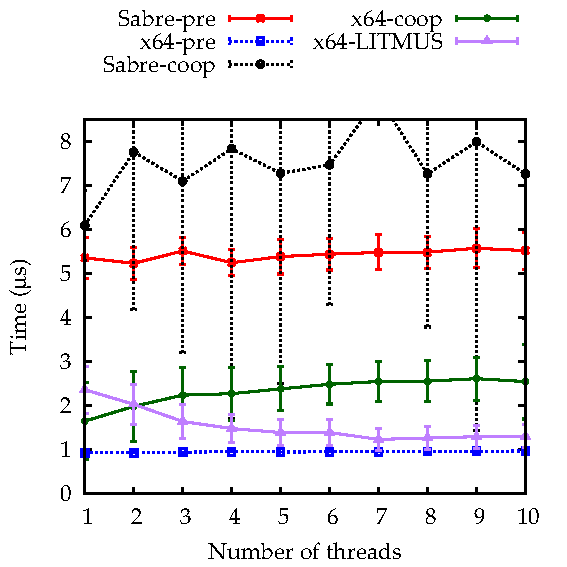
\includegraphics{edf}
    \caption{Execution time of \selfour user-mode EDF scheduler compared to
             kernel scheduler in \textsc{x64} LITMUS$^{RT}$.}
    \label{f:edf}
\end{figure}

\section{Multiprocessor benchmarks}

We run two multicore benchmarks, the first evaluating multicore throughput of the MCS kernel versus the
baseline kernel, the second based on our shared server \gls{AES} case study to demonstrate the
multicore model. 

We run multiprocessor benchmarks on two of our platforms, \textsc{Sabre} and \textsc{x64}. Both 
are symmetric multiprocessors with four cores. 

\subsubsection{Throughput}

We run a multicore throughput benchmark to show that our MCS model
avoids introducing scalability problems on multiple cores compared to the baseline kernel.
We modify the
existing multicore IPC throughput benchmark for \selfour to run on the MCS kernel. 
At time of writing, only \textsc{x64} and \textsc{sabre} have \selfour multiprocessor support, 
consequently these are the platforms used for the benchmark.

The existing multicore benchmark measures IPC throughput of a client and server, both 
pinned to the same processor, sending fastpath, 0 length IPC messages of via \call
and \replyrecv. One pair of client and server is set up per core. Both threads are
the same priority and the messages are 0 length. Each thread spins for a random amount
with an upper bound \textit{N} between each subsequent IPC. As \textit{N} increases so does
IPC throughput, as fewer calls are made.

We modify the benchmark such that each server thread is passive on the MCS kernel.
Results are displayed in \Cref{f:evaluation-smp} and show a minor impact on IPC throughput
for high values of \textit{N}. Scalability is not impacted on \textsc{sabre}, but is on \textsc{x64},
with the curve flattening slightly more aggressively on the MCS kernel
due to the fastpath overhead. This is expected as the MCS model only introduces extra 
per-core state, with no extra shared state between cores.

\begin{figure}[ht] 
    \centering
    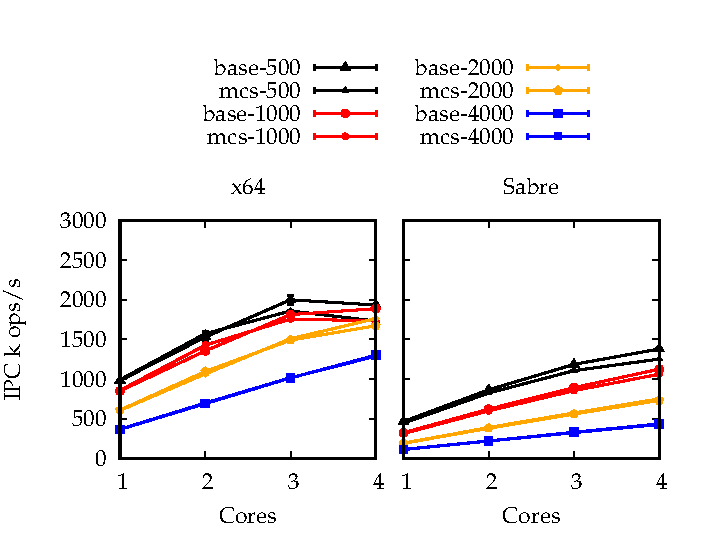
\includegraphics{smp}
    \caption{Results of the multicore IPC throughput benchmark, baseline \selfour vs MCS. 
        Each series is named \textit{name-N}, where \textit{name} is \textit{base} and \textit{mcs} for 
        the baseline and MCS kernel respectively, and \textit{N} is the upper
        bound on the number of cycles between each IPC for that series.}
    \label{f:evaluation-smp}
\end{figure}

\subsubsection{Shared server}

We adapt our \gls{AES} case study (\cref{s:server-isolation}) to demonstrate how our MCS model 
applies to multiprocessors. The AES server is configured without a timeout fault handler, and
we run two variants. 

\begin{description}
    \item[Single:] the AES server has a single passive thread, which waits on a single endpoint
        and migrates to the core of the active client over IPC, effectively serialising access to the server.
        Consequently, \cref{f:evaluation-smp-aes} shows there is no gain in throughput when further cores are
        added. 
    \item[Multiple:] the AES server has one passive thread per core, and an endpoint is set up for
        each core, demonstrating a parallel server. Due to minimal bottlenecks in the stateless 
        AES server, this results in near perfect scalability.
\end{description}

\begin{figure}[ht] 
    \centering
    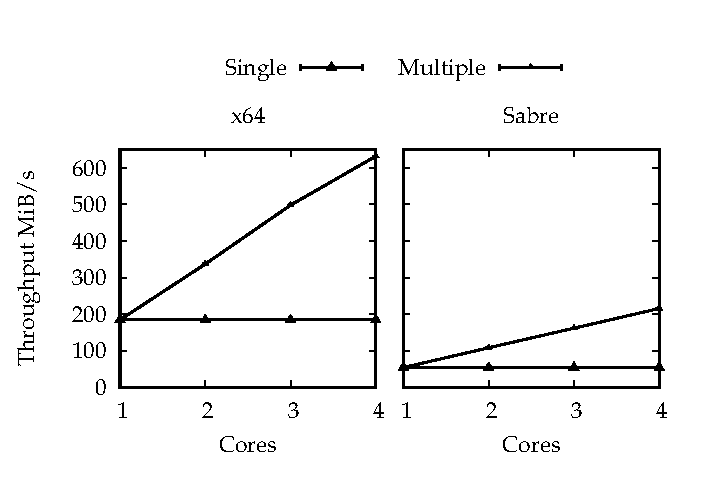
\includegraphics{smp_aes}
    \caption{Results of the AES shared server multicore case study. \emph{Single} shows results for a 
        passive server thread migrating between cores to service clients, while \emph{Multiple} has one
        passive server thread per core. For both series, the number of clients is equal to the number of
        cores and each client requests 1MiB of data encrypted. }
    \label{f:evaluation-smp-aes}
\end{figure}

\section{Summary}

All in all, we have demonstrated via micro- and macro- benchmarks that our overheads are
reasonable given the speed of the baseline kernel and the extent of the provided
functionality. 

Through two system benchmarks and one shared-server benchmark, we have shown
that our approach guarantees processor isolation and that threads cannot exceed
their budget allocation via their scheduling context. Additionally, we have
shown that isolation can be achieved in a shared server via a timeout fault
handler and implemented several alternatives for handling such faults,
demonstrating the feasibility of the model. 

Policy freedom is maintained although we provide a fixed-priority scheduling in the kernel, the primitives are provided are sufficient to implement user-level schedulers, 
as demonstrated through the static, mixed-criticality and EDF scheduler
implementations. 

Finally we have demonstrated that the model works for multiprocessors,
incurring no great scalability penality over baseline \selfour, 
and showing how passive servers which migrate across cores on \gls{IPC}
